\documentclass[10pt]{article}\usepackage[margin=.7in]{geometry}\usepackage{graphicx}\begin{document}\section*{UInt64 doubling correspondence}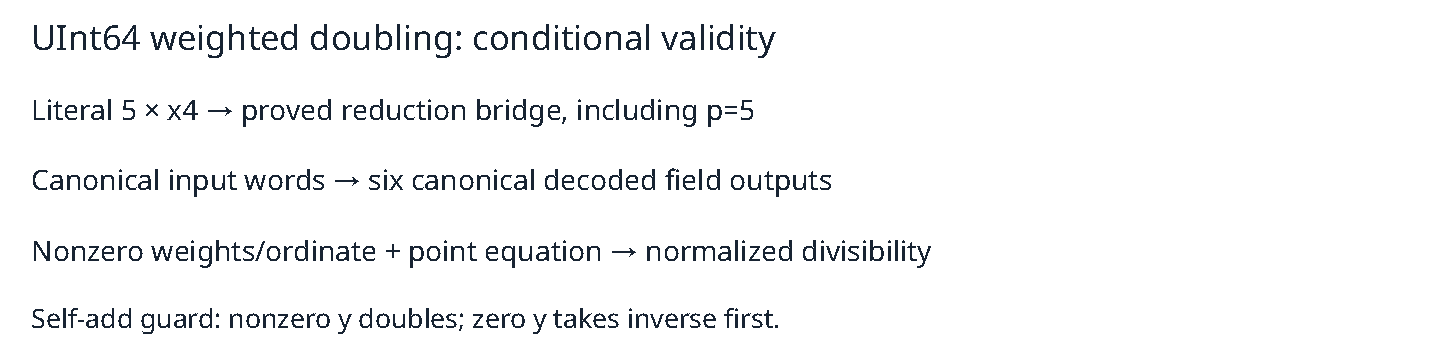
\includegraphics[width=\linewidth]{figure.pdf}
Five Lean theorems compile. Separate controls and axiom readback return exit zero. All six literal payload words are canonical and decode to the independently reviewed weighted field formula; conditional normalized validity follows by composition.

\paragraph{Literal-five boundary} The source multiplier5 is not a canonical leaf when p=5. A bounded UInt64 lemma proves equality after replacing that multiplier with its residue in the proof expression. The literal source payload remains unchanged, and the original prime range is preserved.

\paragraph{Assumptions} Prime $5\le p<2^{31}$, canonical four curve coefficients and four input coordinates. Validity additionally requires nonzero decoded z,w,y,2 and the normalized point equation. The field2 condition is explicit though redundant for this prime range.

\paragraph{Controls and branches} Nonunit weights at p5 instantiate the full composed theorem, with exact payload outputs checked. Self-add doubling and zero-ordinate inverse precedence are verified. The p5 polynomial fixture is not a nonsingular curve or a validation of normalization preprocessing.

\paragraph{Evidence and scope} Failed proof/control attempts are retained; final proof, controls and readback pass with standard Lean axioms. No compiler, counter, class-sum or whole-walk claim. REPORT.md, sources.json and native receipts retain details. Independent review pending; no repository edits or scientific trials.
\end{document}